\documentclass[12pt,a4]{article}




\usepackage{graphicx,amsmath,amssymb,amsthm, boxedminipage,xcolor}

%\usepackage[lined,boxed]{algorithm2e}

\usepackage{algorithm}
\usepackage{algpseudocode}

%\usepackage{algorithmic}
\usepackage{algpseudocode}
\usepackage{amsmath}
\usepackage{graphics}
\usepackage{epsfig}

\newtheorem{theorem}{Theorem}[section]
\newtheorem{proposition}[theorem]{Proposition}
\newtheorem{lemma}[theorem]{Lemma}
\newtheorem{corollary}[theorem]{Corollary}
\newtheorem{definition}[theorem]{Definition}

\newtheorem*{theorem*}{Theorem}
\newtheorem*{lemma*}{Lemma}
\newtheorem*{proposition*}{Proposition}


\newtheorem{exercise}[theorem]{Exercise}
\newtheorem{exerciseD}[theorem]{*Exercise}
\newtheorem{exerciseDD}[theorem]{**Exercise}

\let\oldexercise\exercise
\renewcommand{\exercise}{\oldexercise\normalfont}

%\let\oldexerciseD\exerciseD
%\renewcommand{\exerciseD}{\oldexerciseD\normalfont}

%\let\oldexerciseDD\exerciseDD
%\renewcommand{\exerciseDD}{\oldexerciseDD\normalfont}

\newcommand{\E}{\mathbb{E}}
%\newcommand{\nth}[1]{#1^{\textsuperscript{th}}}
\newcommand{\scalar}[2]{\ensuremath{\langle #1, #2\rangle}}
\newcommand{\floor}[1]{\left\lfloor #1 \right\rfloor}
\newcommand{\ceil}[1]{\left\lceil #1 \right\rceil}
\newcommand{\norm}[1]{\|#1\|}
\newcommand{\pfrac}[2]{\left(\frac{#1}{#2}\right)}
\newcommand{\nth}[1]{#1^{\textsuperscript{th}}}
\newcommand{\core}{\textnormal{core}}



\newif\ifsolution

\solutionfalse

\newcommand{\answer}[1]{
\ifsolution
{\color{blue} #1}
\else
\fi
}



\newcommand{\poly}{\textnormal{poly}}
\newcommand{\quasipol}{\textnormal{quasipol}}
\newcommand{\ssubexp}{\textnormal{stronglySubExp}}
\newcommand{\wsubexp}{\textnormal{weaklySubExp}}
\newcommand{\simplyexp}{\textnormal{E}}
\newcommand{\expo}{\textnormal{Exp}}



\newcommand{\N}{\mathbb{N}}
\newcommand{\nn}{\mathbb{N}_0^n}
\newcommand{\R}{\mathbb{R}}
\newcommand{\Z}{\mathbb{Z}}


\definecolor{darkgreen}{rgb}{0,0.6,0}


\date{}

\title{
  Mathematical Foundations \\of \\Computer Science\\
  \vspace{3mm}
{\normalsize CS 499,	Shanghai Jiaotong University,  Dominik Scheder}
}

\begin{document}

\maketitle

%\begin{quotation}
%  You are welcome to discuss the exercises in the discussion
%  forum. Please take them serious. Doing the exercises is as important
%  than watching the videos.
%
%  I intentionally included very challenging exercises and marked them
%  with one or two ``$*$''. No star means you should be able to solve
%  the exercises without big problems once you have understood
%  the material from the video lecture. One star means it requires 
%  significant additional thinking. Two stars means it is not 
%  unlikely that you will fail to solve them, even once you have understood
%  the material and thought a lot about the exercise. Don't feel bad
%  if you fail. Failure is part of learning.
%
%  This is the first time this course is online. Thus there might be mistakes
%  (typos or more serious conceptual mistakes) in the exercises. I will be 
%  grateful if you point them out to me!
%\end{quotation}





\setcounter{section}{5}


\section{Graph Theory Basics}



\begin{itemize}
 \item Homework assignment published on Monday, 2018-04-02.
 \item Submit first solutions and questions by Sunday, 2018-04-08, 12:00, by
 email to dominik.scheder@gmail.com and to the TAs.
 \item You will receive feedback by Wednesday, 2018-04-11.
 \item Submit final solution by Sunday, 2018-04-15 to me and the TAs.
\end{itemize}


Let $G = (V, E)$ and $H = (V', E')$ be two graphs. A {\em graph isomorphism} from $G$ to $H$
 is a bijective function $f: V \rightarrow V'$ such that
 for all $u,v \in V$ it holds that $\{u,v\} \in E$ if and only if $\{f(u),f(v)\} \in E'$. 
 If such a function exists, we write $G \cong H$ and say that $G$ and $H$ are {\em isomorphic}.
 In other words, $G$ and $H$ being isomorphic means that they 
 are identical up to the names of its vertices.
 
Obviously, every graph $G$ is isomorphic to itself, because the identity function $f(u) = u$ is an
isomorphism. However, there might be several isomorphisms $f$ from $G$ to $G$ itself.
We call such an isomorphism from $G$ to itself an {\em automorphism} of $G$.

\begin{exercise}
For each of the graphs below, compute the number of automorphisms it has.
\begin{center}
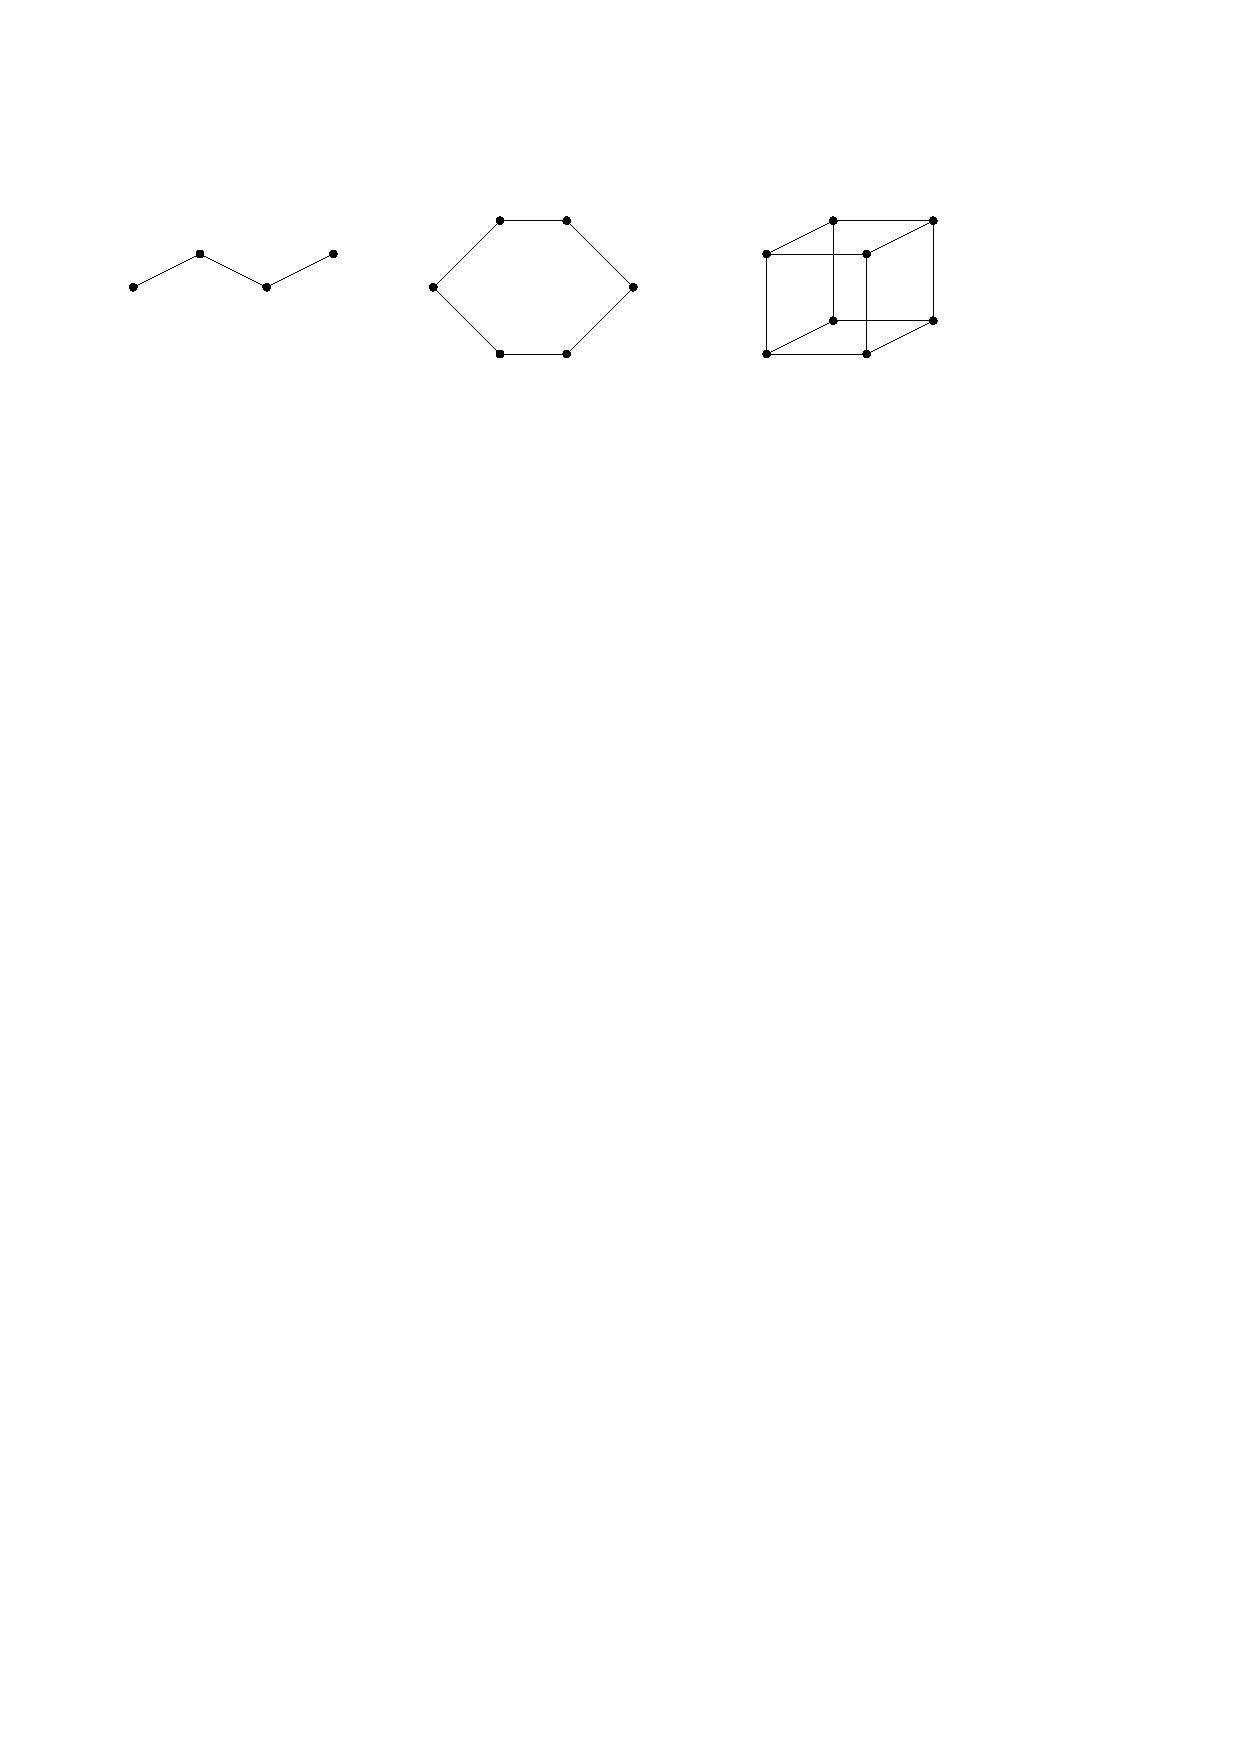
\includegraphics[width=\textwidth]{figures/graphs-number-of-automorphisms.pdf}
\end{center}
Justify your answer!
\end{exercise}


\par
\par
\par
Answer: 2, 12, 48\\
\textbf{Proof.} First we give each vertex of graphs an ID for convenience.
\begin{figure}[hpbt]
\begin{center}
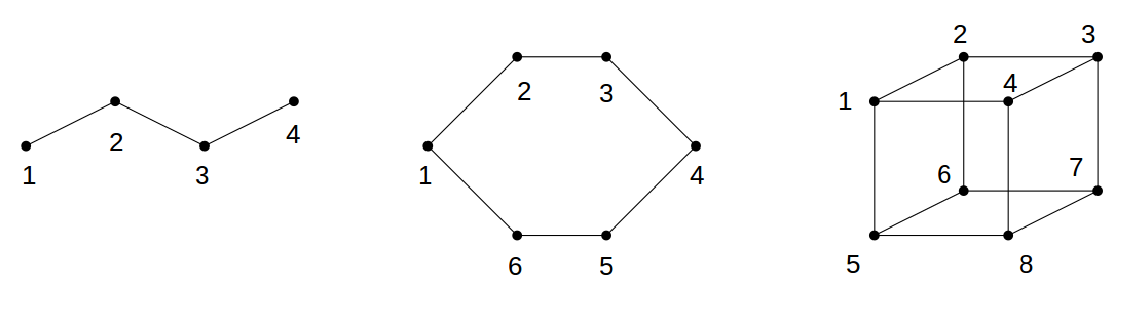
\includegraphics[width=0.8 \textwidth]{ex6-1_img.png}
\end{center}
\end{figure}

In the first graph, there are two vertex $1,4$ with only one degree, which means their corresponding vertices in automorphism have only one degree. Therefore we have 
$$f(1)=1, f(4)=4$$ 
or 
$$f(1)=4, f(4)=1$$
Either case the automorphism can be determined. There are $2$ automorphic graphs. The functions are
$$f_1=\{\{1,1\}, \{2,2\}, \{3,3\}, \{4,4\}\}$$ 
$$f_2=\{\{1,4\}, \{2,3\}, \{3,2\}, \{4,1\}\}$$
\par In the second graph, we take vertex $1$ and $2$ and the edge between them $e_{12}$. The corresponding edge in the automorphism can be $e_{12},e_{21}, e_{23}, e_{32},..., e_{61},e_{16}$. Once the corresponding edge of $e_{12}$ is determined, the automorphism is determined. So there are  $12$ automorphisms.

\par In the third graph, we will illustrate our methods by an example first. If we take $e_{12}$ and choose $e_{43}$ as its mapping in automorphism, there are $4$ choices left for $e_{14}$, as $e_{14}$ can be $e_{14}, e_{23}, e_{48}, e_{37}$. Once the mappings of $e_{12}$ and $e_{14}$ are determined, the automorphism is determined. We have $12$ choices for $e_{12}$ and $4$ choices for $e_{14}$, so there are $48$ automorphisms.

Consider the $n$-dimensional Hamming cube $H_n$. This is the graph with vertex
set $\{0,1\}^n$, and two vertices $x,y \in \{0,1\}^n$ are connected by an edge if 
they differ in exactly one edge. For example, the right-most graph in the figure above
is $H_3$.

\begin{exercise}
   Show that $H_n$ has exactly $2^n \cdot n!$ automorphisms.
   Be careful: it is easy to construct $2^n \cdot n!$ different automorphisms. It is 
   more difficult to show that there are no automorphisms other than those.
\end{exercise}

\begin{exercise}


ex 6-2


\end{exercise}

\begin{proof}

First we choose a vertex in $G$ to be corresponding to our first vertex, say vertex $1$. There is $2^n$ ways. Note that $n-1$ adjacent vertexes to it can uniquely form a hyperplane and they are all symmetrical. So we arrange them to the adjacent vertexes and there is only $n!$ ways since all the hyperplanes are unique.
As a result, the number of automorphism is $2^nn!$.
\end{proof}



A graph $G$ is called {\em asymmetric} if the identity function $f(u) = u$ is the 
only automorphism of $G$. That is, if $G$ has exactly one automorphism.

\begin{exercise}
   Give an example of an asymmetric graph on six vertices.
\end{exercise}





\begin{figure}[hpbt]


\begin{center}


    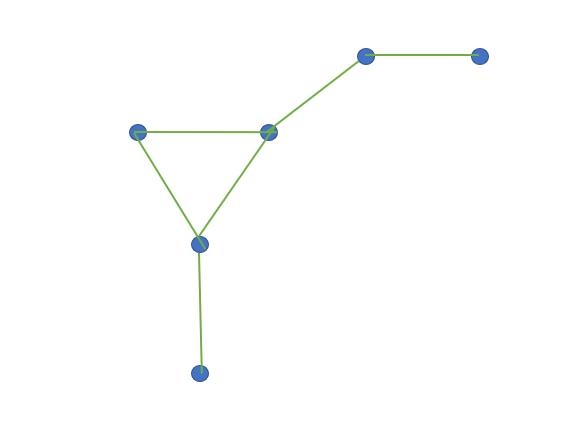
\includegraphics[width=0.3 \textwidth]{lym.png}


\end{center}


\end{figure}


\begin{exercise}
  Find an asymmetric tree.
\end{exercise}

\begin{exercise}
ex 6-4
\end{exercise}

%%%%%%%%%%%%%%%%%%%%%%%%%%%%%%%%%%

\begin{figure}[hpbt]
\begin{center}
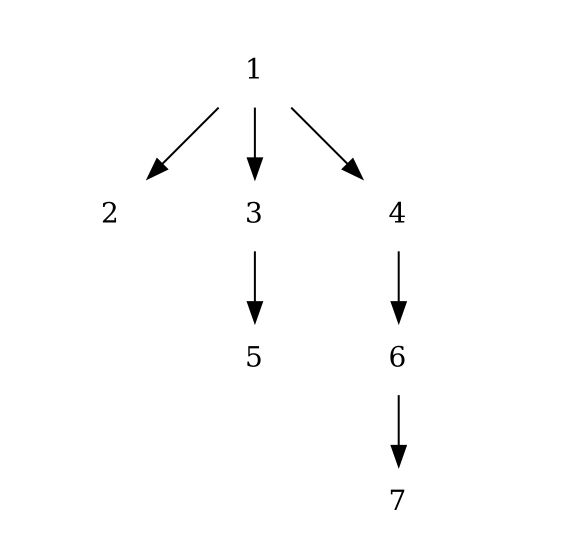
\includegraphics[width=0.3 \textwidth]{Ex6-4.png}
\end{center}
\end{figure}


For a graph $G = (V,E)$, let $\bar{G} := \left(V, {V \choose 2} \setminus E \right)$ denote
its {\em complement graph}.
\begin{center}
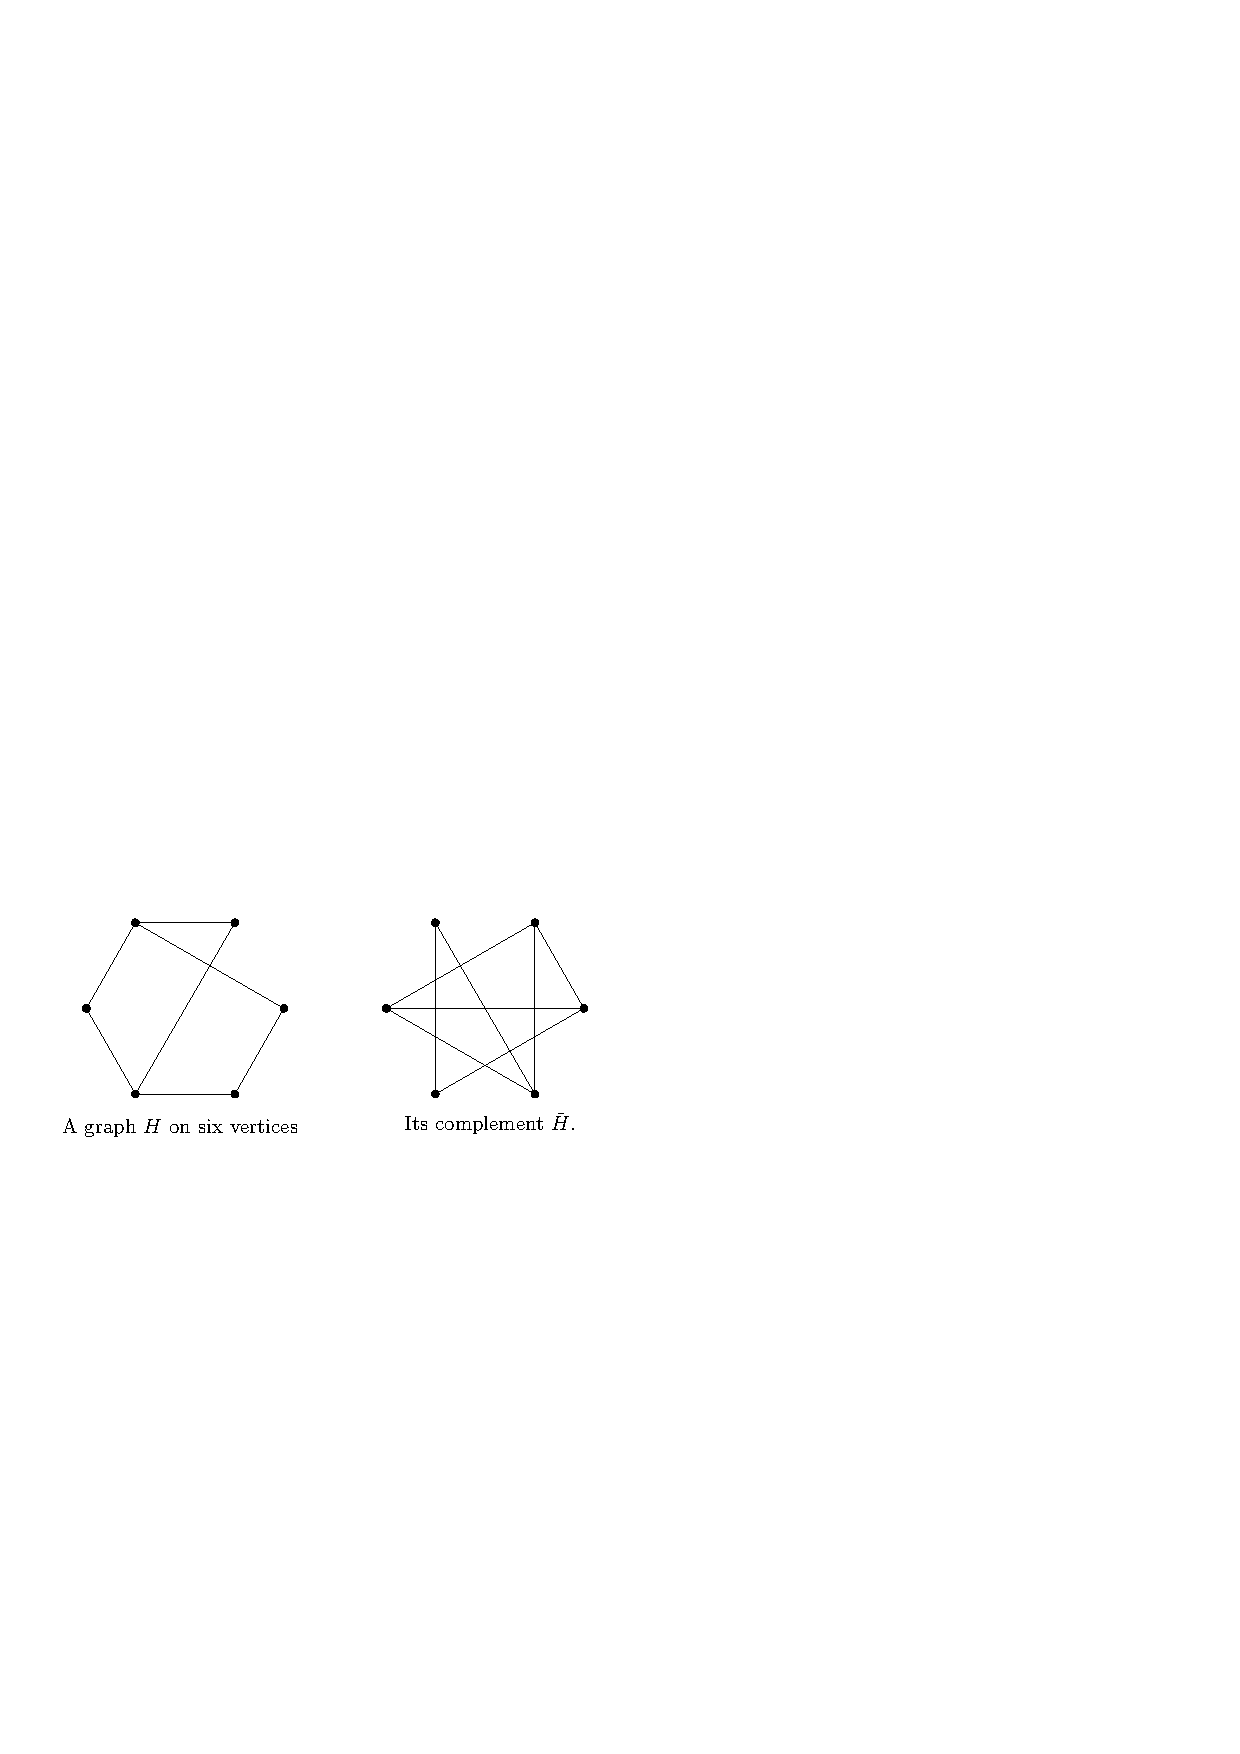
\includegraphics[width=0.5\textwidth]{figures/graph-complement.pdf}
\end{center}
We call a graph {\em self-complementary} if $G \cong \bar{G}$. The above graph
is not self-complementary. Here is an example of a self-complementary graph:
\begin{center}
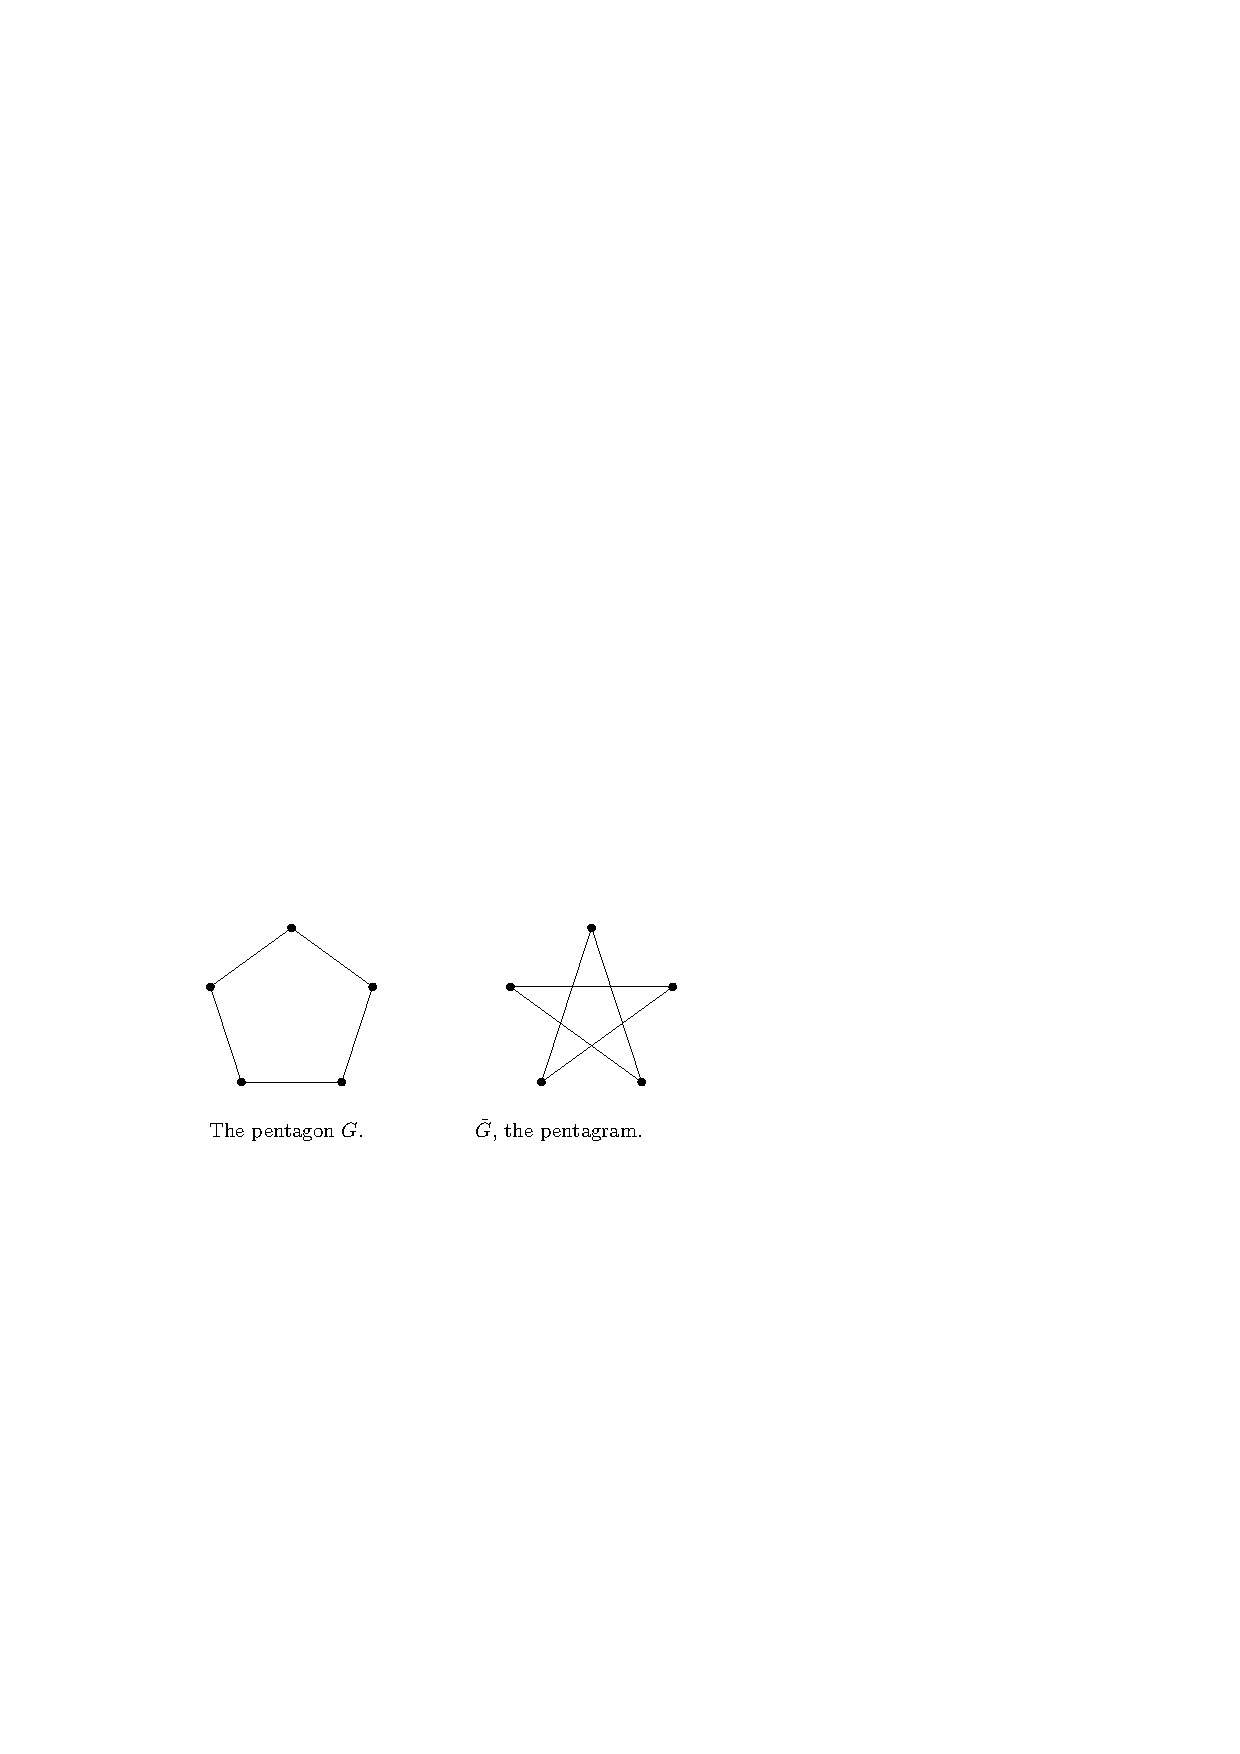
\includegraphics[width=0.5\textwidth]{figures/pentagon-pentagram.pdf}
\end{center}


\begin{exercise}
   Show that there is no self-complementary graph on $999$ vertices.
\end{exercise}

%\begin{exercise}
%ex6-5
%\end{exercise}

\begin{proof}
Since the edges of a graph and its automorphism are same, total edges of the complete graph be composed of both of them must be even.However, a graph consists of 999 vertices has $C_{999}^2=498501$ edges, which is odd. So there is no self-complementary graph on 999 vertices.
\end{proof}

%\begin{exercise}
%ex6-6
%\end{exercise}

%Answer: $n=4k\: or\: 4k+1$
%\begin{proof}
%Maybe we can prove it by adjacent matrix.
%\end{proof}


\begin{exercise}
 Characterize the natural numbers $n$ for which there is a self-complementary
 graph $G$ on $n$ vertices. That is, state and prove a theorem of the form
 ``There is a self-complementary graph  on $n$ vertices if and only if 
 $n$ \texttt{ <put some simple criterion here>}.''
\end{exercise}



The criterion we find is:
\par
There is a self-complementary graph on $n$ vertices if and only if $n=4k$ or $n=4k+1$ where $k \in \mathbb{N}$.
\begin{proof}
There are $n \choose 2$ edges in a complete graph of $n$ vertices, which means the sum of the edges of a graph and its complementary graph is $n \choose 2$.
$$|E|+|E'|={n \choose 2}$$
For a self-complementary graph, there is $|E| = |E'|$.
$$|E|=\frac{1}{2} {n \choose 2}=\frac{n(n-1)}{4}$$
Obviously, the edges of a graph should be an integer and as $n$ and $n-1$ must be one odd and one even, so 
$$n \equiv 0 \mod 4$$ 
or 
$$n-1 \equiv 0 \mod 4$$
these two conditions can be rewritten as
$$n=4k ~or~ 4k+1, \textbf{where} ~ k\in \mathbb{N}$$ 
Then we will prove the condition is sufficient by finding a self-complementary graph for $n=4k$ and $n=4k+1$.

\par
For $n=4k$, we split the vertices to $4$ groups with $k$ vertices in each group, as the following picture shows.

\begin{figure}[hpbt]
\begin{center}
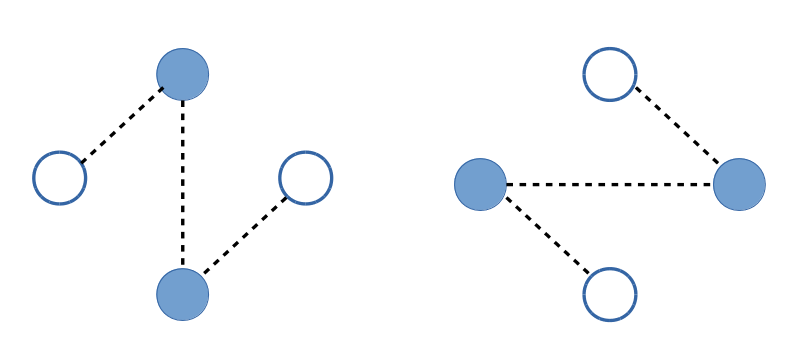
\includegraphics[width=0.6 \textwidth]{Ex6-6_1.png}
\end{center}
\end{figure}

A group in blue stands for the vertices in group is "fully connected", that is, $ \{u, v\} \in E $ for any two $u,v \in V_{blue}$. 
\par A group in white stands for there is no edge between any two vertices in white group. $ \{u, v\} \not \in E$ for any two $u,v \in V_{white}$.
\par The dot lines stands for there is an edge for any two vertices from groups the line connecting to. $ \{u, v\} \in E$ for $u \in V_1$, $v \in V_2$. 
\par 
The complementary graph of the left graph is the right graph. And we can easily see that they are isomorphic. So there is a self-complementary graph for $n=4k$.


For $n=4k+1$, we add one more vertex $x$ to the graph we found for $n=4k$.
\begin{figure}[hpbt]
\begin{center}
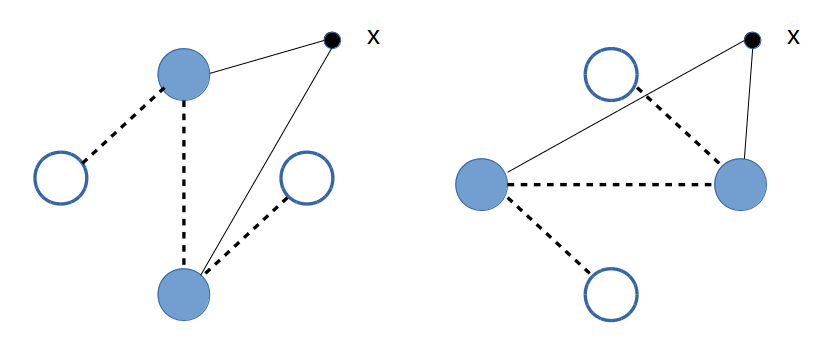
\includegraphics[width=0.6 \textwidth]{Ex6-6_2.png}
\end{center}
\end{figure}
Then we put edges between $x$ and vertices in blue groups. The black line stands for there is an edge between the vertex and any verterx in the group. $\{x, u\} \in E$ for any $u \in V_{blue}$.
\par
The graph's complementary graph is shown as well. We observe that they are isomorphic. So there is also a self-complementary graph for $n=4k+1$.   

\par So there is a self-complementary graph on $n$ vertices if and only if $n=4k$ or $n=4k+1$ where $k \in \mathbb{N}$.
\end{proof}


\end{document}